% !TEX root = ./paper.tex



\subsection{Methodology}

Our objective is to evaluate whether our design and implementation are indeed
fast, flexible and does not conflict with several commercial and open-source
middleboxes. Moreover, we expect to showcase and compare TCPLS's functionalities
such as the App-level connection migration, the failover mechanism or the
bandwidth aggregation capability. We discuss them against the state
of the art designs, such as mvfst~\cite{mvfast}, quicly~\cite{quicly},
msquic~\cite{msquic}, MPTCP~\ref{mptcp}, pquic~\cite{pquic},
quic-go~\cite{quic-go} and MPQUIC~\ref{mpquic}.

%TODO do we also evelatuate security? with a simple proof and discussion?
To evaluate the performance (Section~\ref{sec:perf}) and middlebox traversal
(Section~\ref{sec:middlebox}), we deploy a testbed composed of three machines with Intel Xeon CPU E5-2630
2.40GHz, 16 Threads, at least 16GB RAM, running Debian with 5.9 and
5.7 kernels. Two of these machines play the role of Client and Server,
while one is the Network Simulator (NS). Each machine is equipped with an
Intel XL710 2x40GB NIC, directly connected as shown in
Fig.~\ref{fig:perf_testbed}.
Each device is configured to maximize its performances, with a single TCP connection
reaching 22 Gbps with a 1500 Bytes MTU and linerate (i.e., 40 Gbps) when
using jumbo frames.

\begin{figure}[!t]
  \begin{center}
    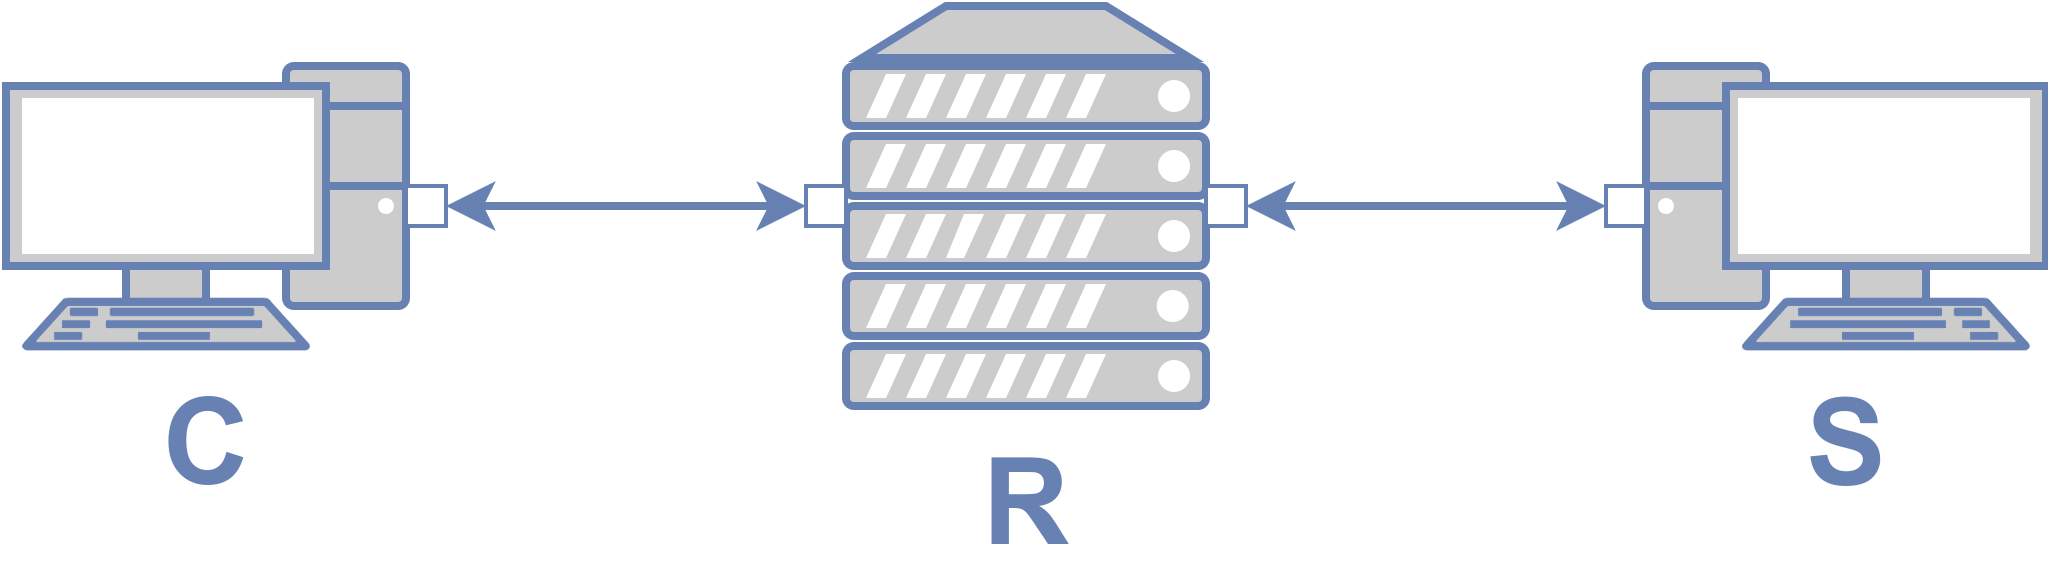
\includegraphics[width=6cm]{figures/testbed.png}
  \end{center}
  \vspace{-0.5cm}
  \caption{Performance Measurements Setups. C = Client. S = Server. MB = Middlebox.}
  \label{fig:perf_testbed}
    \vspace{-0.5cm}
\end{figure}

The traffic exchanged by client and server has to go through the NS first.

To evaluate TCPLS's functionalities, we rely on reproducible network
experimentations with Mininet~\cite{mininet}. Our objective is to compare the
behaviour of TCPLS with the state of the art, and to make it easily
reproducible for future works, as the quic implementations continue to evolve.

\subsection{Capability Comparison}

Table~\ref{table:tcplsvsquic} compares the features supported by
\tcp, \tls/\tcp, QUIC and \tcpls. QUIC and \tcpls are very similar in their
capabilities. They mainly differ in their semantic. \tcpls's semantic is to let
the applications make the decision, and we design its API to fulfill this goal.
That is, the meaning of \tcpls is to offer advanced, extensible and secure
transport-layer functionalities on top of \tcp, while exposing a simple but
powerful API to let the application composes the properties its transport should
have.

Note that several of the features suggested by \tcpls are also suggested on \tcp or
QUIC via research works such as a new socket API for explicit multipath for
\tcp\cite{hesmans2016enhanced}, or eBPF plugins in
QUIC~\cite{de2019pluginizing}.

\begin{table}
  \small
  \begin{tabular}{lcccc}
    \toprule
    & \tcp & \tls/\tcp & QUIC & \tcpls \\
    \midrule
    Transport reliability & \checkmark & \checkmark &
    \checkmark & \checkmark \\
    Message conf. and auth.&  \xmark & \checkmark & \checkmark & \checkmark \\
    Connection reliability (failover) &  \xmark & \xmark & (\checkmark) & \checkmark \\
    0-RTT & \checkmark & (\xmark) & \checkmark  & \checkmark \\
    Session Resumption & \xmark & \checkmark & \checkmark & \checkmark \\
    Connection Migration & \xmark & \xmark & \checkmark & \checkmark \\
    \multicolumn{5}{l}{Application-exposed features} \\
    \hspace{2em} Streams & \xmark & \xmark & \checkmark & \checkmark \\
    \hspace{2em} Happy eyeballs & \xmark & \xmark & \xmark & \checkmark \\
    \hspace{2em} Explicit Multipath & \xmark & \xmark & \xmark & \checkmark \\
    \hspace{2em} App-level Con. migration & \xmark & \xmark & \xmark & \checkmark \\
    \hspace{2em} Pluginization & \xmark & \xmark & \xmark & (\checkmark) \\
    Resilience to HOL blocking & \xmark & \xmark & \checkmark  & \checkmark \\
    Secure Connection Closing & \xmark &  \xmark & \checkmark & \checkmark \\
    \bottomrule
  \end{tabular}
  \caption{Protocol features comparison. (\xmark) means that the feature is
    available, but not straightforward to use. (\checkmark) means that the
  feature is partially available and under development.}
  \label{table:tcplsvsquic}
\end{table}

\subsection{Performance}
\label{sec:perf}

We perform a throughput evaluation of \tcpls and compare it to several major
QUIC implementations: mvfst~\cite{} from Facebook, msquic~\cite{} from Microsoft
and quicly~\cite{} from Fastly. Our choice of QUIC implementations was mainly
influenced by the availability of a client/server perf tool specifically
engineered for a throughput evaluation. A second criterion was the advancement
of the implementation and the quality of the code. We hope to avoid most of the
bugs negatively impacting their results by selecting the QUIC implementation
that show advanced features and testings. A third criterion was the development
language used. \tcpls is written in C, and we prefer to compare it against QUIC
implementation written in a language compiled by clang or gcc. Mvfst, msquic
and quicly meet these criteria. Besides, mvfast and quicly also support generic
segmentation offload, which is a plus for throughput experimentation, since those
implementions would speed up thanks to the offloading UDP segmentation and
checksum computation available on our NICs. We use the implementation's
client/server perf tools as is, exploiting the optional arguments provided
by their interface to increase the throughput but drawing the line there. That
is, we do not change their implementation.

Figure~\ref{fig:perf} shows several interesting results. First, while
offering similar (and more) capabilities than what QUIC is providing today,
\tcpls is also more than twice faster than the strongest evaluated QUIC
implementation (quicly) over CPU limited experimentations. We evaluate \tcpls
in four different settings: with a path mtu of 1500 or 9000, and with failover
enabled or not. The failover functionality is an internal stack feature that
provides session reliability, which increases the number of syscalls that TCPLS
makes by exchanging TCPLS-level record acknowledgments. We currently send an ack
for every 16 received records, or when we receive 15 times the maximum TLS
payload, or when a timer expires. Reducing the frequency would improve
throughput at the price of a slower recovery in case of network failure.

TLS/TCP's experiments uses \texttt{picotls}'s client/server implementation with
the same commit than our initial fork for TCPLS. TLS/TCP's lower performance results
can be explained by the receiving buffer size provided to \texttt{read()}, which
is hardcoded to 16384 bytes. This choice makes the client suffers from
fragmentation and cannot exploit the zero-copy code path provided by the
library, which \tcpls can do with a larger read buffer. At first, we may think
that this is not a fair comparison, however the devil is in the detail. In our
implementation, the application developers cannot touch \texttt{read()}'s
interface. That is, the application developer cannot missuse the relationship
between TLS and TCP by creating fragmented records and doing unecessary copies
to handle those fragments. TCPLS's design and implementation may try to prevent
such fragmentation to happen, by first, having a sufficiently large read buffer
size. Second, by deciphering a record only when we known we received the record
entirely. TLS/TCP record fragmentation is provided by TLS libraries as a
usability feature that spares the application developers to care about TLS
details, at the cost of slower performance. \tcpls allows the application
developers to ignore TLS details without missusing the interface,
which is the reason this comparison is interesting. Moreover, but this has not
yet been implemented, it could be interesting to match the TLS record size to
the congestion window to deliver faster the data to the application whe the
network is under congestion.


\begin{figure}[!t] \begin{center}
    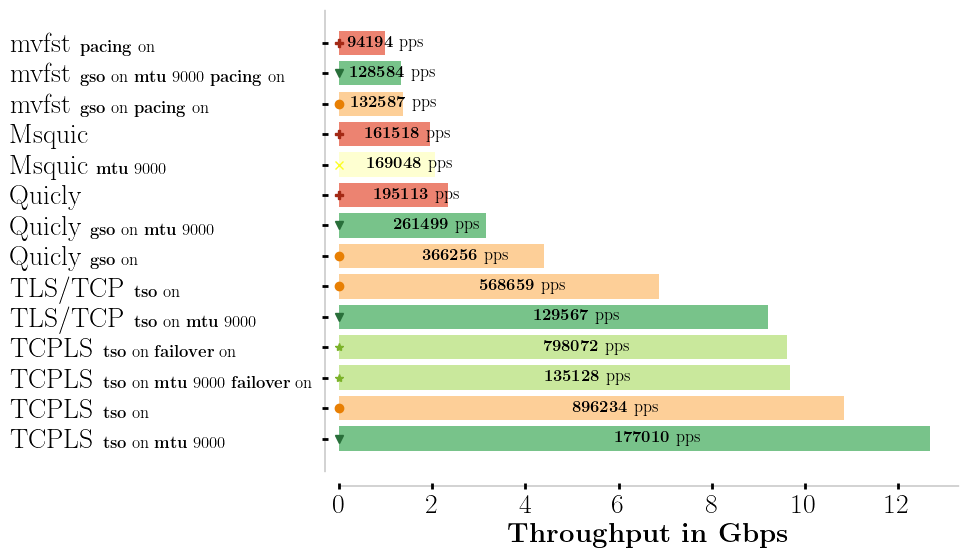
\includegraphics[width=\columnwidth]{figures/perf_analysis.png} \end{center}
  \caption{Throughput measurements of various QUIC stacks, TLS/TCP and TCPLS}
  \label{fig:perf} \end{figure}

\subsection{Middlebox Interferences}

When deploying a novel protocol, different middlebox interferences may arise
depending on the changes introduced in the packets wire image. In this
regard, \tcpls comes with two novel \tls extensions: \tcpls and \join.
We discuss the potential issues and contermeasures below.

If a clients attempts to open a \tcpls to in the presence of a \tls termination
proxy, it sends a ClientHello that includes the \tcpls extension. If the proxy
does not support \tcpls, it replies with a ServerHello message that does not
include the \tcpls extension. From this point, the client implicitely fallback
to \tls, and continues with the handshake.

Certain legacy \tls server implementations are known not to implement the \tls
specification properly and might abort connections when receiving unknown TLS
extensions. Analogous behavior has been observed in overly restrictive stateful
firewalls.  To ensure connectivity in the presence of such policies, \tcpls
implements an explicit fallback mechanism. If a device sends a \tcp \rst in
response to the \tcpls-setup ClientHello, or silently discards it, the client
attempts at negotiating a second non-\tcpls \tls connection, either immediately
or after a timeout. Similarly, a \tcpls \join extension might be blocked on the
path. In this case, the subflow attachment is canceled, and the application
is directly notified to be able to react appropriatly.

We tested \tcpls against several opensource and commercial stateful firewalls
implementations (i.e., pfSense, IPFire, Cisco ASAv) and found no interferences.

\subsection{Bandwidth Aggregation}

\begin{figure}[!t] \begin{center}
    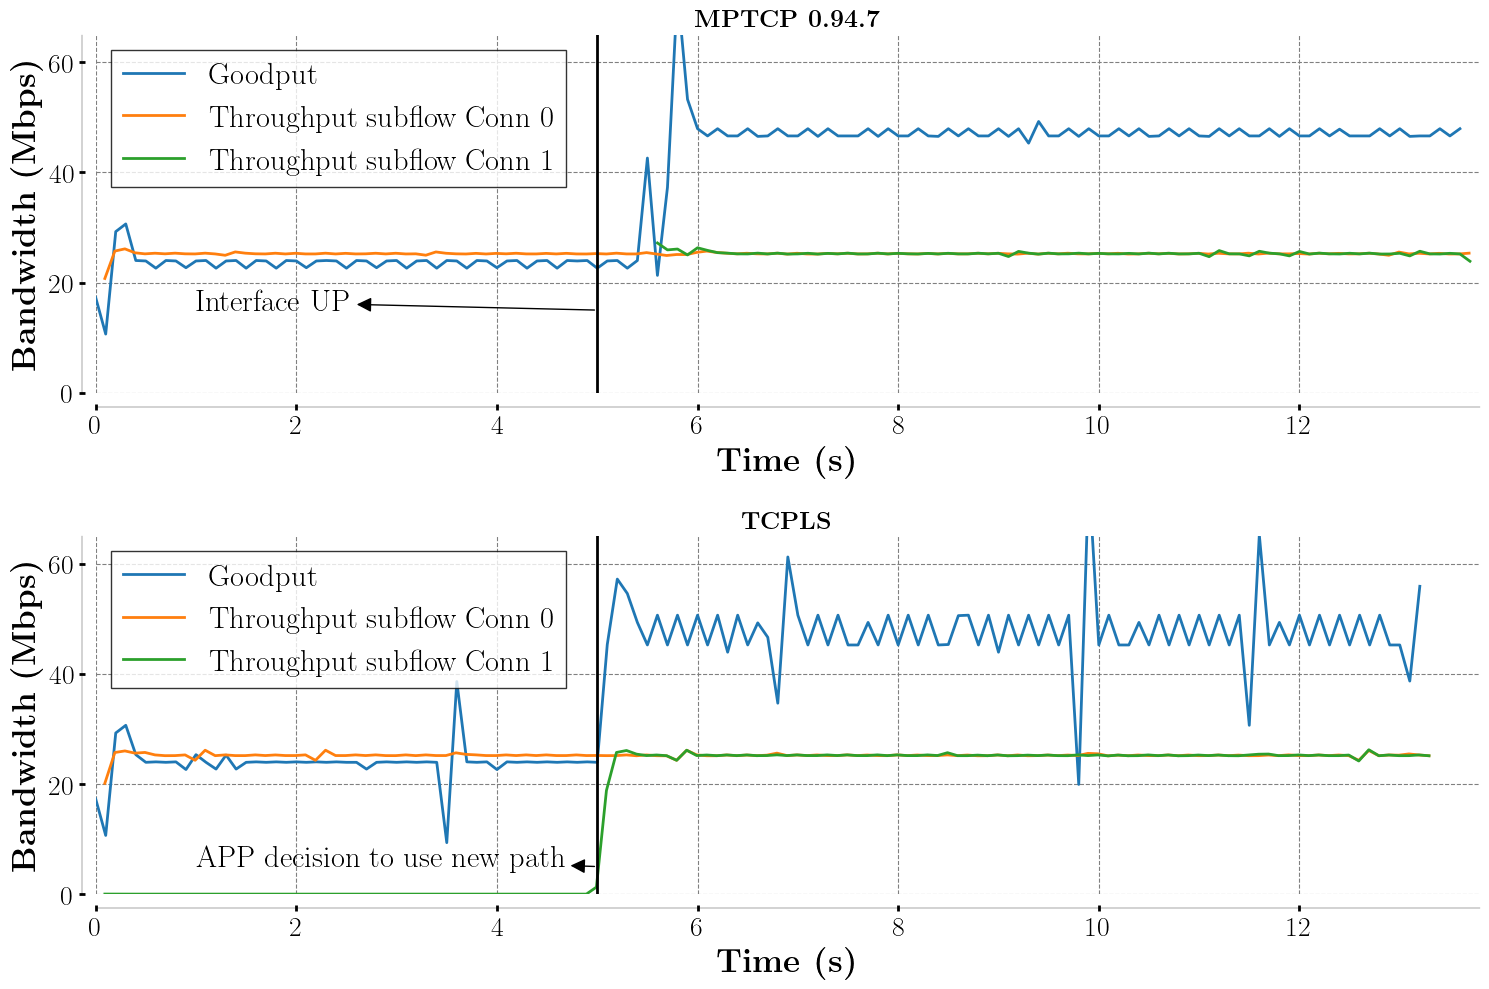
\includegraphics[width=\columnwidth]{figures/aggregate_dual.png}
  \end{center} \caption{Bandwidth aggregation comparison between MPTCP and
    TCPLS.} \end{figure}

\subsection{Application-level migration}

Detailler pourquoi on a besoin du controle applicatif pour la migration, et à
quels cas du monde réels ils s'appliquent


Figure~\ref{fig:conn_migration} shows the result of an Application-level
connection migration demo using the API (i.e., it is left to the
application to decide when to migrate, and we expose a simplistic code flow to
perform it). In this experiment, we use an IPMininet network~\cite{ipmininet, jadin2020educational}
composed of a client and a server with a dual-stack of IPs. One path within the
network is composed of OSPF routers with IPv4 only, and one path is composed of
OSPF6 routers IPv6 only. We configure the bandwidth to 30Mbps, the lowest delay
to the v4 link. Our application
downloads a 60 MB file from a server and migrates to the v6 connection in
the middle of the download.

Triggering the connection migration involves chaining 5 API calls:
first, \texttt{tcpls\_handshake()} configured with handshake properties announcing a JOIN over the v6 connection id. Then, the creation of a new stream
\texttt{tcpls\_stream\_new()} for the v6 connection id, finally followed by the attachment of this new stream \texttt{tcpls\_streams\_attach()} and the secure closing of the v4 \tcp connection using \texttt{tcpls\_stream\_close()}. Following these events, the server seamlessly switches the path while looping over \texttt{tcpls\_send} to send the file content. Note that all the events trigger callbacks on the server side, to let the server react appropriately if other requirements need to be fulfilled.

\tcpls's application connection migration takes advantage of multipath to offer
a smooth handover to applications, which QUIC cannot do at the moment.

\begin{figure}[!t]
  \centering
  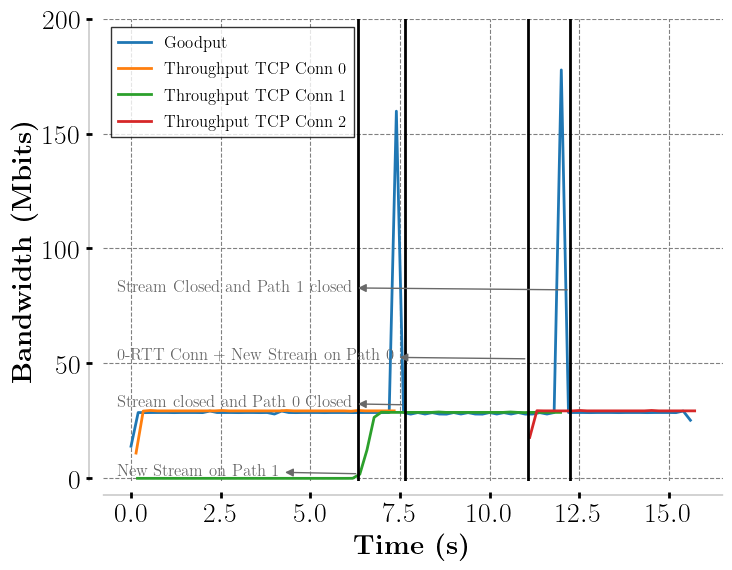
\includegraphics[width=6cm]{figures/migration.png}
  \caption{Application-level connection migration during a 60MB file download.}
  \label{fig:conn_migration}
\end{figure}

\subsection{Failover}

1) analyse du temps de recovery pour different type de cassure, et comparaison avec mptcp
2) discuter une propriété de "connection reliability" => ca casse, on restabilise le plus vite possible
3) montrer que le path manager est important pour cette propriété, et que ce n'est pas encore au point pour mptcp, mpquic, etc

Mptcp overhead: 1.0744997978210449
TCPLS overhead: 1.0994282363439873
MPTCP overhead/TCPLS overhead:              0.9773259975513828


\begin{figure}[!t]
  \begin{center}
    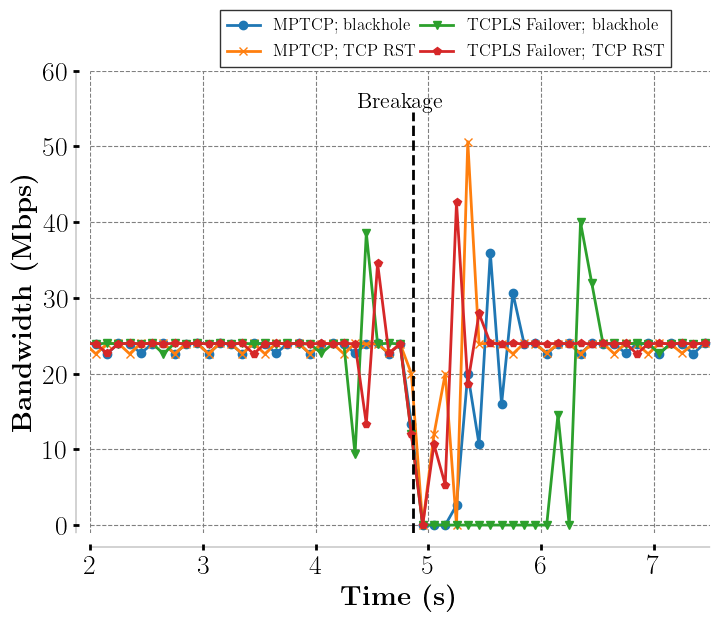
\includegraphics[width=6cm]{figures/breakage_analysis.png}
  \end{center}
  \caption{Recovery speed analysis.}
\end{figure}


\begin{figure}[!t]
  \begin{center}
    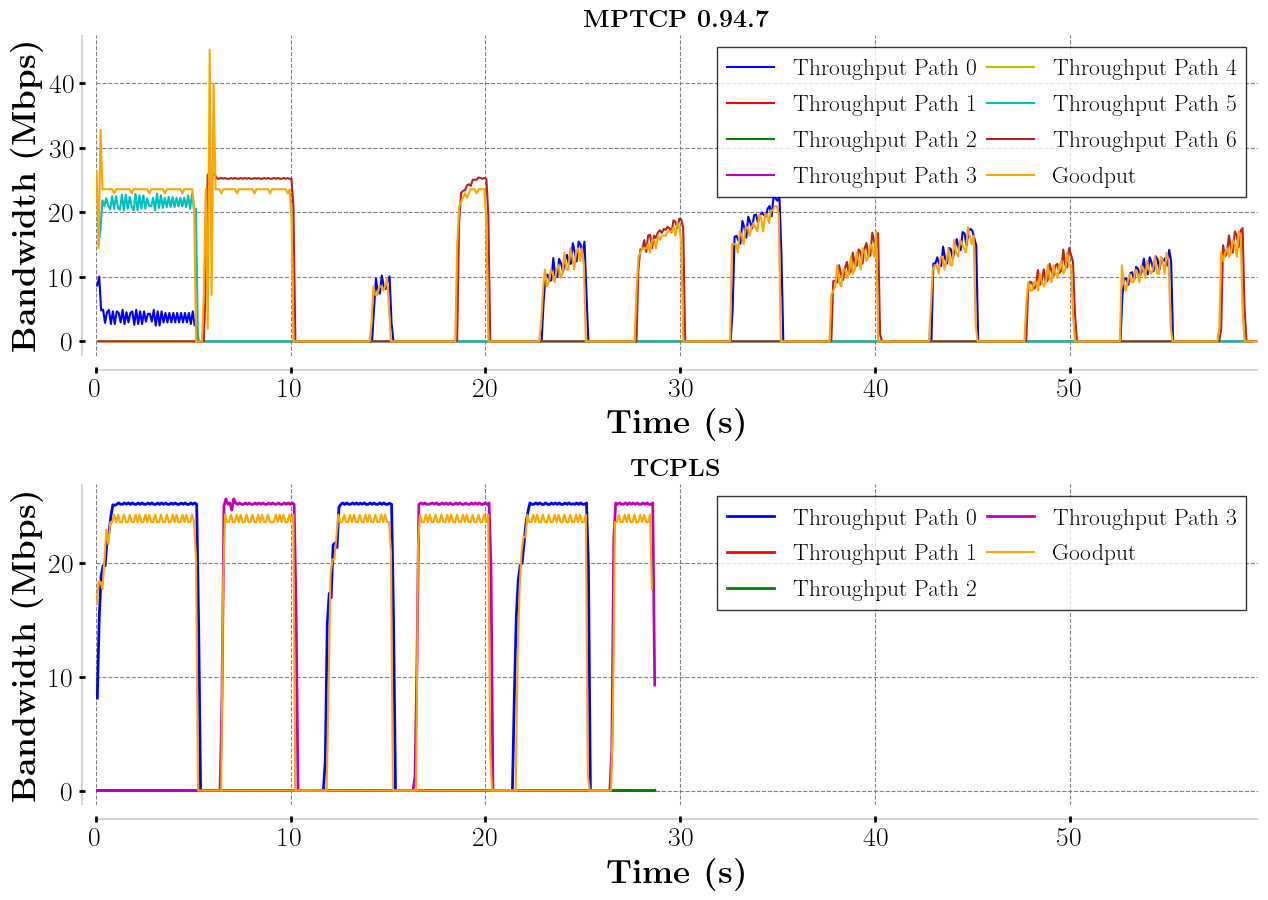
\includegraphics[width=6cm]{figures/tcpls_mptcp.png}
  \end{center}
  \caption{Connection reliability: influence of the path manager and congestion
  control.}
\end{figure}



\subsection{Dynamically extending TCPLS}

The TCPLS streams enable new use case. Obviously, a TCPLS application can
create and use different streams to carry data. However, since these streams
are generic, they can also be used by the TCPLS implementation itself to
exchange control information. To demonstrate the versatily of these control
streams, we extended TCPLS to enable a server to push a different congestion
control scheme to a specific client over an existing TCPLS session. Recent
work on restructuring congestion control has proposed a generic architecture
for congestion controllers \cite{narayan2018restructuring}. 
During the last years, the Linux kernel developpers have relied on eBPF
to make the Linux TCP/IP stack \cite{brakmo2017tcp,tran2020beyond} easier
to extend. Since Linux kernel version 5.xx, $Emery$ an application can inject
a different congestion control scheme entirely implemented using eBPF. A similar approach was proposed in Pluginizing QUIC~\cite{de2019pluginizing}.
We leverage these new eBPF capabilities to
demonstrate the feasibility of injecting and
updating a congestion control scheme during a TCPLS session.

We perform our experiment using Mininet over a 100 Mbps emulated link that has a 60 msec delay. Figure~\ref{fig:vegasCubic} shows a client that uses the TCP Vegas \cite{10.1145/190314.190317} congestion control scheme to upload a file. This TCLPS session fully uses the bottleneck link. After some time, another client starts an upload, but using the CUBIC congestion controller \cite{rfc8312}. This results in an unfair distribution of the bandwidth. The server then sends the eBPF bytecode of the CUBIC congestion control scheme to the TCP Vegas client that injects it in its kernel and the unfairness disappears.

\begin{figure}[!t]
  \begin{center}
    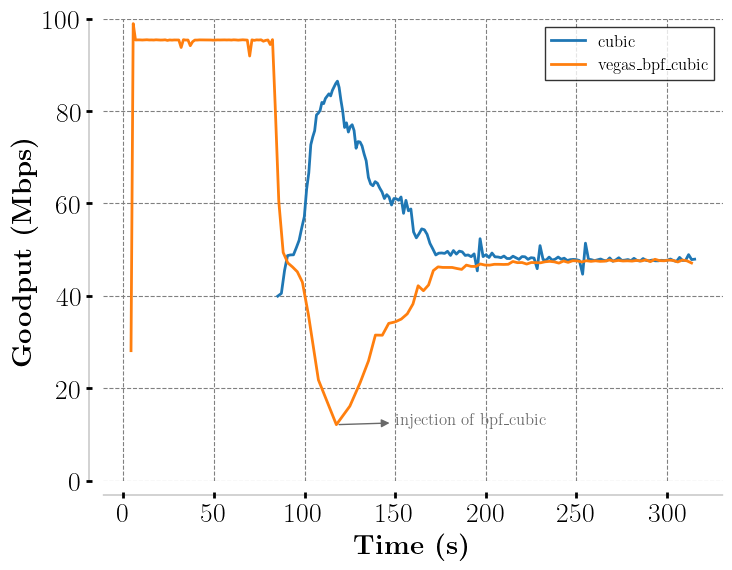
\includegraphics[width=6cm]{pretty_plotify/plots/vegas_cubic.png}
  \end{center}
  \caption{TCPLS hosts can exchange congestion control schemes and activate them during a TCPLS session.}
  \label{fig:vegasCubic}
\end{figure}











Injecter un control de congestion, montrer que les perf s'améliorent
